\hypertarget{IndependenceTest_8h}{
\section{Independence\-Test.h File Reference}
\label{IndependenceTest_8h}\index{IndependenceTest.h@{IndependenceTest.h}}
}


This graph shows which files directly or indirectly include this file:\begin{figure}[H]
\begin{center}
\leavevmode
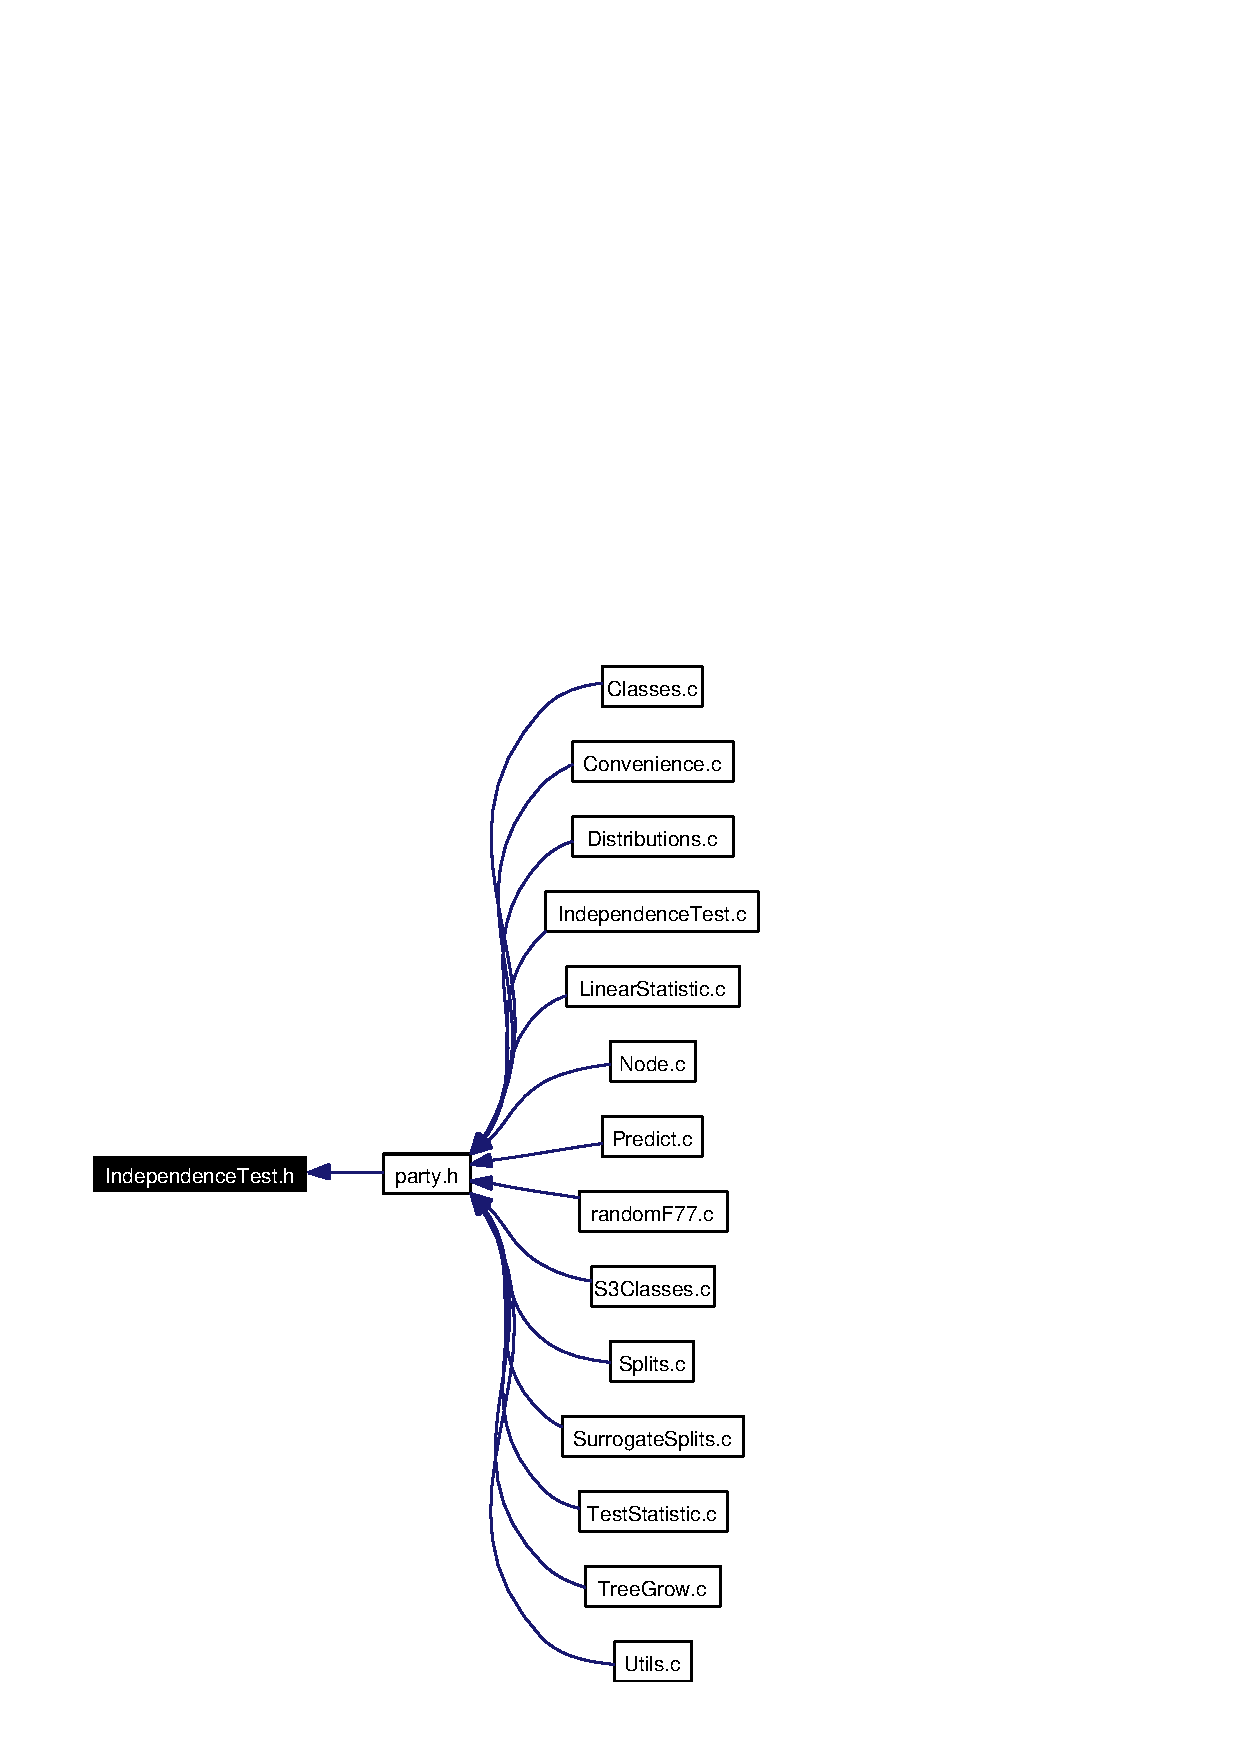
\includegraphics[width=185pt]{IndependenceTest_8h__dep__incl}
\end{center}
\end{figure}
\subsection*{Functions}
\begin{CompactItemize}
\item 
void \hyperlink{IndependenceTest_8h_a0}{C\_\-Global\-Test} (SEXP learnsample, SEXP weights, SEXP fitmem, SEXP varctrl, SEXP gtestctrl, double minsplit, double $\ast$teststat, double $\ast$criterion)
\item 
void \hyperlink{IndependenceTest_8h_a1}{C\_\-Teststat\-Pvalue} (const SEXP linexpcov, const SEXP varctrl, double $\ast$ans\_\-teststat, double $\ast$ans\_\-pvalue)
\item 
void \hyperlink{IndependenceTest_8h_a2}{C\_\-Teststat\-Criterion} (const SEXP linexpcov, const SEXP varctrl, double $\ast$ans\_\-teststat, double $\ast$ans\_\-criterion)
\end{CompactItemize}


\subsection{Function Documentation}
\hypertarget{IndependenceTest_8h_a0}{
\index{IndependenceTest.h@{Independence\-Test.h}!C_GlobalTest@{C\_\-GlobalTest}}
\index{C_GlobalTest@{C\_\-GlobalTest}!IndependenceTest.h@{Independence\-Test.h}}
\subsubsection[C\_\-GlobalTest]{\setlength{\rightskip}{0pt plus 5cm}void C\_\-Global\-Test (const SEXP {\em learnsample}, const SEXP {\em weights}, SEXP {\em fitmem}, const SEXP {\em varctrl}, const SEXP {\em gtctrl}, const double {\em minsplit}, double $\ast$ {\em ans\_\-teststat}, double $\ast$ {\em ans\_\-criterion})}}
\label{IndependenceTest_8h_a0}


Perform a global test on independence of a response and multiple inputs \par
 \begin{Desc}
\item[Parameters:]
\begin{description}
\item[{\em learnsample}]an object of class `Learning\-Sample' \item[{\em weights}]case weights \item[{\em fitmem}]an object of class `Tree\-Fit\-Memory' \item[{\em varctrl}]an object of class `Variable\-Control' \item[{\em gtctrl}]an object of class `Global\-Test\-Control' \item[{\em minsplit}]minimum sum of weights to proceed \item[{\em ans\_\-teststat}]return value; vector of test statistics \item[{\em ans\_\-criterion}]return value; vector of node criteria (adjusted) pvalues or raw test statistics\end{description}
\end{Desc}


Definition at line 129 of file Independence\-Test.c.

References AGGREGATED, BONFERRONI, C\_\-Expect\-Covar\-Influence(), C\_\-Lin\-Stat\-Exp\-Cov(), C\_\-Lin\-Stat\-Exp\-Cov\-MPinv(), C\_\-Monte\-Carlo(), C\_\-Sample\-No\-Replace(), C\_\-Teststat\-Criterion(), get\_\-dontuse(), get\_\-dontusetmp(), get\_\-missings(), get\_\-mtry(), get\_\-ninputs(), get\_\-nobs(), get\_\-randomsplits(), get\_\-teststat(), get\_\-testtype(), get\_\-tol(), get\_\-transformation(), get\_\-varmemory(), get\_\-weights(), has\_\-missings(), MONTECARLO, ncol(), nrow(), PL2\_\-expcovinf\-Sym, PL2\_\-inputs\-Sym, PL2\_\-responses\-Sym, PL2\_\-sumweights\-Sym, TESTSTATISTIC, and UNIVARIATE.

Referenced by C\_\-Node(), and R\_\-Global\-Test().

Here is the call graph for this function:\begin{figure}[H]
\begin{center}
\leavevmode
\includegraphics[width=219pt]{IndependenceTest_8h_a0_cgraph}
\end{center}
\end{figure}
\hypertarget{IndependenceTest_8h_a2}{
\index{IndependenceTest.h@{Independence\-Test.h}!C_TeststatCriterion@{C\_\-TeststatCriterion}}
\index{C_TeststatCriterion@{C\_\-TeststatCriterion}!IndependenceTest.h@{Independence\-Test.h}}
\subsubsection[C\_\-TeststatCriterion]{\setlength{\rightskip}{0pt plus 5cm}void C\_\-Teststat\-Criterion (const SEXP {\em linexpcov}, const SEXP {\em varctrl}, double $\ast$ {\em ans\_\-teststat}, double $\ast$ {\em ans\_\-criterion})}}
\label{IndependenceTest_8h_a2}


Computes the test statistic and the node criterion \par
 \begin{Desc}
\item[Parameters:]
\begin{description}
\item[{\em linexpcov}]an object of class `Lin\-Stat\-Expect\-Covar' \item[{\em varctrl}]an object of class `Variable\-Control' \item[{\em ans\_\-teststat;}]return value, the test statistic \item[{\em ans\_\-criterion;}]return value, thep-value\end{description}
\end{Desc}


Definition at line 53 of file Independence\-Test.c.

References C\_\-Teststat\-Pvalue(), and get\_\-pvalue().

Referenced by C\_\-Global\-Test(), and C\_\-Monte\-Carlo().

Here is the call graph for this function:\begin{figure}[H]
\begin{center}
\leavevmode
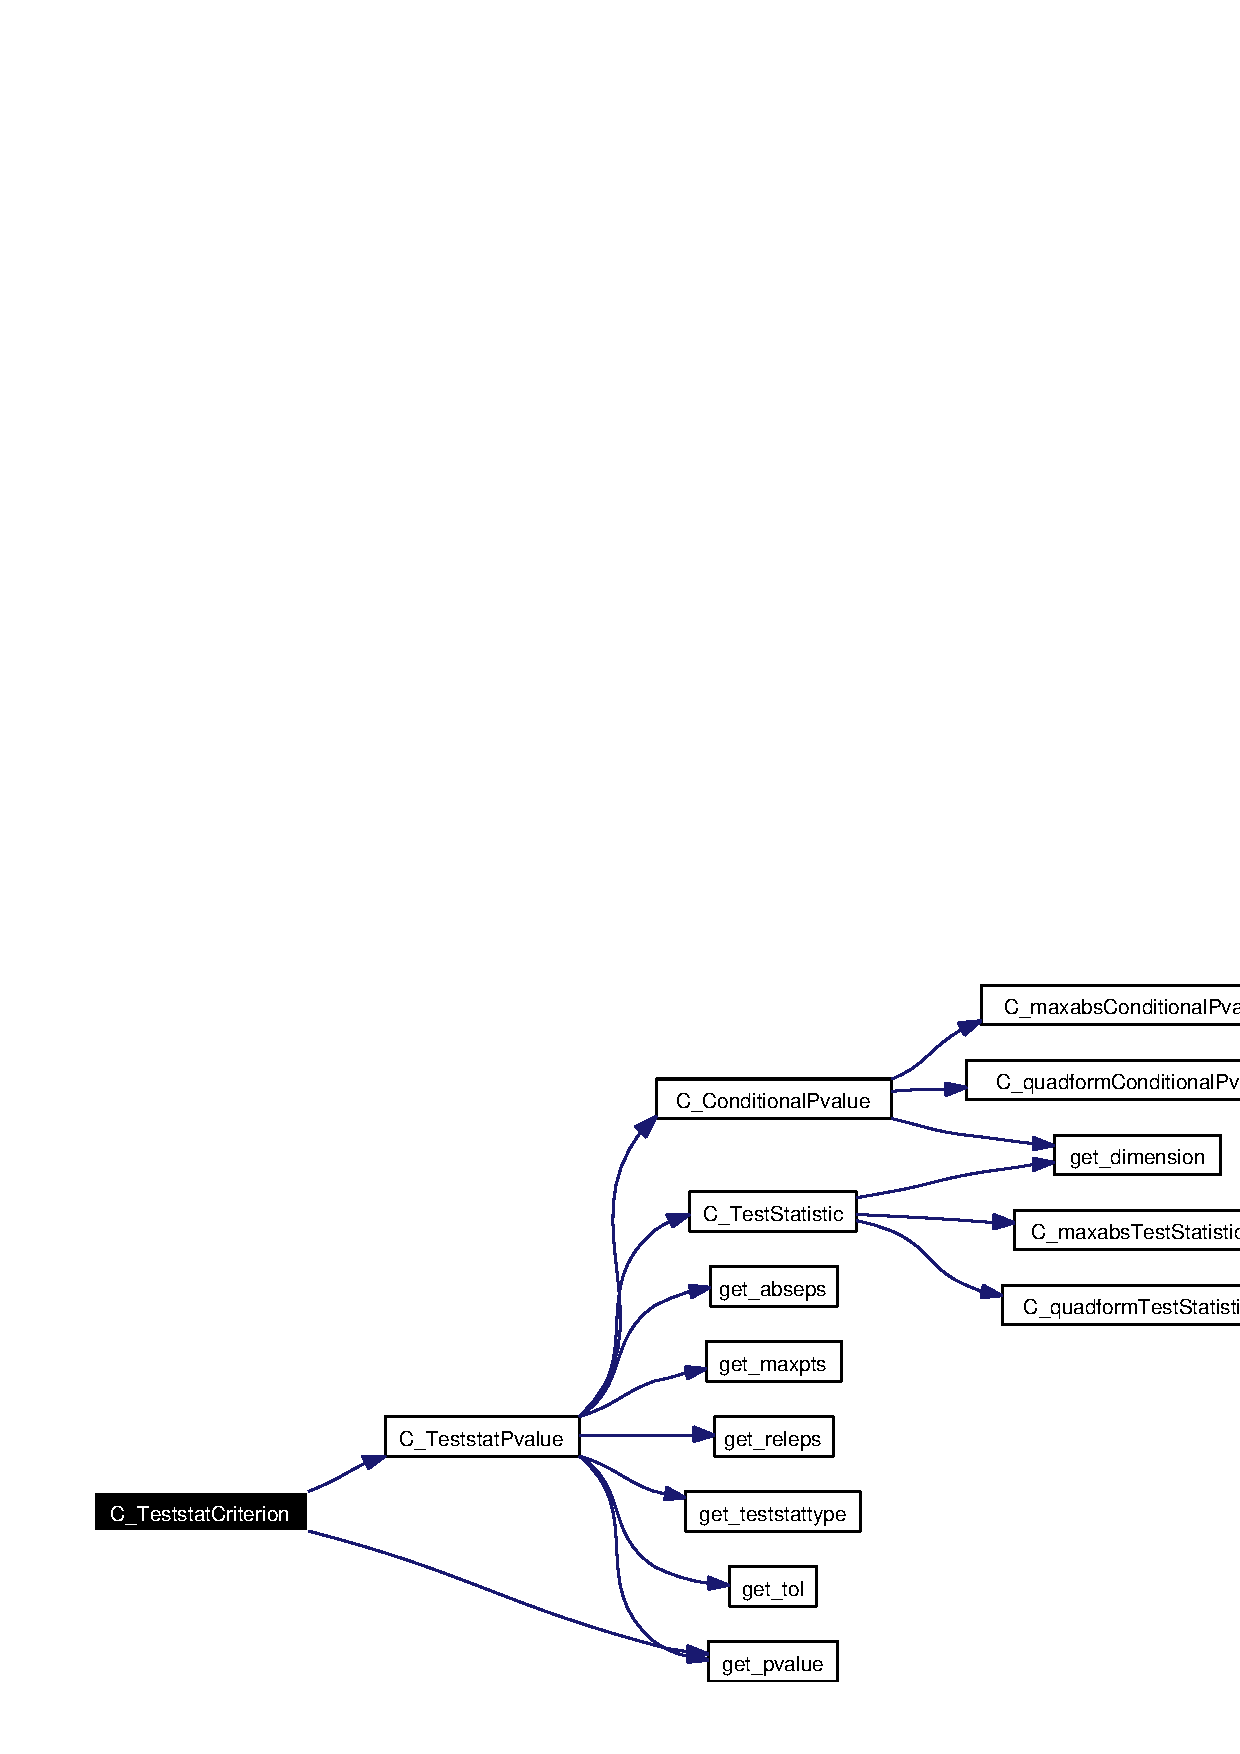
\includegraphics[width=369pt]{IndependenceTest_8h_a2_cgraph}
\end{center}
\end{figure}
\hypertarget{IndependenceTest_8h_a1}{
\index{IndependenceTest.h@{Independence\-Test.h}!C_TeststatPvalue@{C\_\-TeststatPvalue}}
\index{C_TeststatPvalue@{C\_\-TeststatPvalue}!IndependenceTest.h@{Independence\-Test.h}}
\subsubsection[C\_\-TeststatPvalue]{\setlength{\rightskip}{0pt plus 5cm}void C\_\-Teststat\-Pvalue (const SEXP {\em linexpcov}, const SEXP {\em varctrl}, double $\ast$ {\em ans\_\-teststat}, double $\ast$ {\em ans\_\-pvalue})}}
\label{IndependenceTest_8h_a1}


Computes the test statistic and, if requested, the corresponding P-value for a linear statistic \par
 \begin{Desc}
\item[Parameters:]
\begin{description}
\item[{\em linexpcov}]an object of class `Lin\-Stat\-Expect\-Covar' \item[{\em varctrl}]an object of class `Variable\-Control' \item[{\em ans\_\-teststat;}]return value, the test statistic \item[{\em ans\_\-pvalue;}]return value, the p-value\end{description}
\end{Desc}


Definition at line 21 of file Independence\-Test.c.

References C\_\-Conditional\-Pvalue(), C\_\-Test\-Statistic(), get\_\-abseps(), get\_\-maxpts(), get\_\-pvalue(), get\_\-releps(), get\_\-teststat(), and get\_\-tol().

Referenced by C\_\-Independence\-Test(), and C\_\-Teststat\-Criterion().

Here is the call graph for this function:\begin{figure}[H]
\begin{center}
\leavevmode
\includegraphics[width=359pt]{IndependenceTest_8h_a1_cgraph}
\end{center}
\end{figure}
